%! program = pdflatex

%
%  Master Thesis von Dirk Breuer
%
%  Created by Dirk Breuer on 2008-06-02.
%  Copyright (c) 2008 Dirk Breuer. All rights reserved.
%
% only4mac: makeindex Master\ Thesis.nlo -s nomencl.ist -o Master\ Thesis.nls

% header inkludieren. Beinhaltet Pakete und Layoutanweisungen
%!TEX root = /Users/dbreuer/Documents/Work/_FH/_Master/master_thesis/Main/Master Thesis.tex

%%% PREAMBLE

\documentclass[12pt,
               headsepline,
               DIV14, % Seitenränder festlegen
               BCOR5mm, % Bindekorrektur
               a4paper,
               oneside,
               cleardoublestandard,
               openany,
               bibtotoc,
               liststotoc,
               halfparskip,
               pointlessnumbers,
               final
               ]{scrbook}

% Paket für Zeilenabstände
\usepackage{setspace}
\raggedbottom

\usepackage{scrpage2}
\pagestyle{scrheadings}
\clearscrheadfoot
\cfoot{\pagemark}
% \ihead{\headmark}
\ohead{\headmark}
% \automark{section}

% include XMP-Metadata
\usepackage{xmpincl} 
\includexmp{std/metadata}

% Wie viele Ebenen im Inhaltsverzeichnis?
\setcounter{tocdepth}{3}

% Bis zu welcher Ebene sollen die Abschnitt nummeriert werden
\setcounter{secnumdepth}{3}

% Grafiken und Farbe
\usepackage[pdftex]{graphicx} % for graphic handling
\usepackage[usenames,dvipsnames,pdftex]{color} % for color handling
% Einige Farben
\definecolor{lightgray}{gray}{0.95}
\definecolor{cmd_line}{rgb}{0.4,.8,1}
\definecolor{comment}{rgb}{0.2,0.7,0.5}

% Paket für Rotation
\usepackage{rotating}

% Paket für Listings
\usepackage{listings}
\usepackage{dvsm} % Use DejaVu Sans Mono as Monospace Font
% get closed frames on each page for listings
\usepackage{framed}
\lstloadlanguages{Java,XML,Ruby,HTML}
\newcommand{\listingname}{Listing}
\lstset{
  numbers=left, 
	numberstyle=\ttfamily\tiny, 
	stepnumber=1,
	lineskip=3pt,
	numbersep=5pt,
	language=Java,
	breaklines=true,
	breakautoindent=true,
	postbreak=\space,
	tabsize=2,
	frame=single,
  keywordstyle=\bfseries\color{blue},
  stringstyle=\color{ForestGreen},
	numberfirstline=false,
  commentstyle=\slshape\footnotesize\color{Gray},
  basicstyle=\ttfamily\footnotesize,
  % morekeywords={while,condition,invoke,receive,assign,pipe},
  keywordstyle=[2]\ttfamily\redhighlight,
  keywordstyle=[3]\ttfamily\yellowhighlight,
  keywordstyle=[4]\ttfamily\slshape
}

% bg colored text for highlighting

\newcommand{\redhighlight}[1]{\colorbox{red}{\textcolor{white}{#1}}}
\newcommand{\yellowhighlight}[1]{\colorbox{yellow}{\textcolor{black}{#1}}}

% Listings can be included as following:
% 
% include a file (from line n to m): \lstinputlisting[firstline=n,lastline=m]
% 
% standard listing: \begin{lstlisting} ... \end{lstlisting}
% 
% Inline: \lstinline+code here+

% \lstdefinelanguage{SPARQL}{
%     morekeywords = {PREFIX, SELECT, DISTINCT, WHERE },
%   emphstyle=\itshape %\underbar
%   % emph={[2]mit,sonst},
%   emphstyle=[2]\color{red},
%   % moredelim=[is][\color{green}]{/*}{*/}
% }
% 
% \lstdefinelanguage{Turtle}{
%     morekeywords = {@prefix},
%   emphstyle=\itshape %\underbar
%   % emph={[2]mit,sonst},
%   % emphstyle=[2]\color{red},
%   % moredelim=[is][\color{green}]{/*}{*/}
% }

% Use utf-8 encoding for foreign characters
\usepackage[utf8]{inputenc}

% Paket das die Ausgabefonts definiert
% \usepackage[T1]{fontenc}

% Paket um jede Schriftgröße zuzulassen
% \usepackage{type1cm}

% This is now the recommended way for checking for PDFLaTeX:
\usepackage{ifpdf}

% change enumeration package
\usepackage{enumerate}

% Package for verbatim text
\usepackage{verbatim}
% Notwendiges Paket, um Verbatim in Fußzeilen zu setzen
\usepackage{fancyvrb}
\VerbatimFootnotes

% schoenere Kennzeichnung im Literaturverzeichnis
\usepackage[square,sort]{natbib}
% Festlegung Art der Zitierung - Havardmethode: Abkuerzung Autor + Jahr %
% BibTeX Style nach Norm DIN 1505 %
\bibliographystyle{natdin}

% Schriftstile umsetzen
% \setkomafont{sectioning}{\normalfont\normalcolor\bfseries}
\setkomafont{descriptionlabel}{\normalfont\normalcolor\bfseries}
\setkomafont{captionlabel}{\usekomafont{descriptionlabel}}
\setkomafont{dictumtext}{\normalfont\normalcolor\itshape}
\setkomafont{dictumauthor}{\scshape}

% Hurenkinder und Schusterjungen verhindern
\clubpenalty = 10000
\widowpenalty = 10000
\displaywidowpenalty = 10000

% Paket für die Verwendung von URLs durch den Befehl \url{}
\usepackage{url}

%\usepackage{array}
\usepackage{colortbl}

% Babelpaket für deutsche Bezeichner
\usepackage[ngerman]{babel}

% For syntax Checking
\usepackage{syntonly}
% \syntaxonly % Comment out for Output

\usepackage{makeidx}
% \makeindex

% Mathepakete
\usepackage{amssymb} %maths
\usepackage{amsmath} %maths
\usepackage{amsthm}

% Mathematische Definition
\newtheorem{definition}{Definition}
% \usepackage{mathabx}

% Springt im PDFViewer an die Stelle an der gerade editiert wurde
\usepackage{pdfsync}

% Paket und Einstellungen für das Abkürzungsverzeichnis
\usepackage[norefpage,noprefix,german,intoc]{nomencl}
% Befehl umbenennen in abk
\let\abk\nomenclature
% Deutsche Überschrift
\renewcommand{\nomname}{Abkürzungsverzeichnis}
% Punkte zw. Abkürzung und Erklärung
\renewcommand{\nomlabel}[1]{#1 \dotfill}
% Zeilenabstände verkleinern
\setlength{\nomitemsep}{-\parsep}
% Definiert die Aufteilung im Glossar zwischen Begriffen und Erläuterung
\setlength{\nomlabelwidth}{.25\hsize}
%\makeglossary
\makenomenclature

%Paket für ein deutsches Literaturverzeichnis
\usepackage{bibgerm}

% other commands
\newcommand{\note}[1]{\textbf{#1}}

\pdfpagewidth=\paperwidth \pdfpageheight=\paperheight
\usepackage[pdftex,plainpages=false,pdfpagelabels,
            pdftitle={Konzeption, prototypische Realisierung und szenariobasierte Validierung einer dienstorientierten Multimediaarchitektur},
            pdfauthor={Dirk Breuer - University of Applied Science, Cologne},
            pdfkeywords={Architektur,SOA,Prototyping,COSIMA,Validierung}]{hyperref} % Has to stand at the end of the preamble

%%% END PREAMBLE

%%% BEGIN DOCUMENT
\begin{document}

% Vermeidung von "duplicate page" Fehlern
% siehe: http://theoval.sys.uea.ac.uk/~nlct/latex/pdfdoc/pdfdoc/pdfdoc.html
\pagenumbering{alph}

% Unbeschriftetes Vorblatt
\newpage
\thispagestyle{empty}
\mbox{}

 % Titelseite einbinden
%!TEX root = /Users/dbreuer/Documents/Work/_FH/_Master/master_thesis/Main/Master Thesis.tex

\begin{titlepage}

\begin{center}

%Logo der Fachhochschule Köln
\begin{figure}[!ht]
	\flushleft
		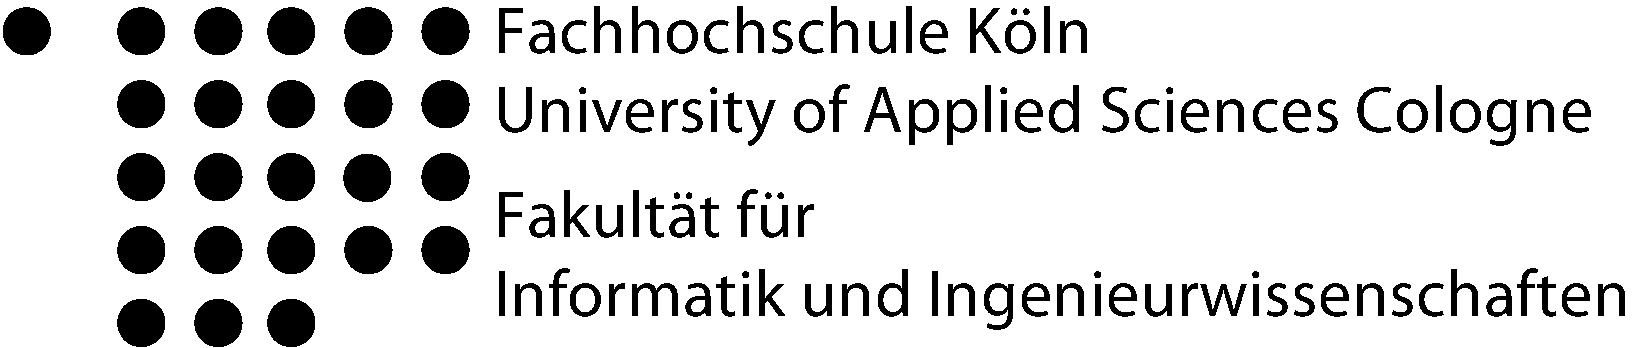
\includegraphics[natwidth=920pt, natheight=95pt, width=.5\textwidth]{images/fh_logo.pdf}
\end{figure}

\vspace{0.5cm}

% Master Thesis 
\begin{Large}
  \textsc{Master Thesis}\\[0.7em]
\end{Large}

%Deutscher Titel
\begin{rmfamily}
  \LARGE
  \textbf{
  Konzeption, prototypische Realisierung und szenariobasierte Validierung einer dienstorientierten Multimediaarchitektur
  }\\
\normalsize
\end{rmfamily}

\vspace{0.5cm}

%Englischer Titel
% \begin{rmfamily}
% \textbf{\LARGE Title in English}\\
% \large with a very\\long subtitle\\
% \normalsize
% \end{rmfamily}
% 
% \vspace{1.2cm}

%ausgearbeitet von...
% \begin{large}
ausgearbeitet von\\ 
% \vspace{0.2cm}
\begin{Large}
Dirk Breuer, 11038920\\Medieninformatik Master\\
\end{Large}
% \end{large}

\vspace{0.6cm}

%zur Erlangung des akademischen Grades...
zur Erlangung des akademischen Grades\\
% \vspace{0.2cm}
\begin{large}
\textsc{Master of Science}\\ 
\end{large}

\vspace{0.4cm}

%vorgelegt an der...
vorgelegt an der\\ 
% \vspace{0.2cm}
\begin{large}
\begin{scshape}
Fachhochschule Köln\\
University of Applied Sciences Cologne\\
Fakultät für Informatik und\\
Ingenieurwissenschaften\\
\end{scshape}
\end{large}

\vspace{0.4cm}

%im Studiengang...
\vspace{0.2cm}
im Studiengang\\ 
\begin{large}
\textsc{Medieninformatik (Master)}
\end{large}

\vspace{0.7cm}

%Autor der Bachelorarbeit und die Prüfer
\begin{tabular}{rl}
         Erster Prüfer: &  Prof. Dr. Mario Winter\\
       							    &  \small Fachhochschule Köln \\[1.0em]
        Zweiter Prüfer: &  Prof. Dr. Kristian Fischer\\
       							    &  \small Fachhochschule Köln \\
\end{tabular}

\vspace{0.5cm}

%Ort, Monat der Abgabe
% \begin{large}
\textsc{Gummersbach, im Dezember 2008}
% \end{large}

\end{center}

\newpage
\thispagestyle{empty}

%Kontaktmöglichkeiten des Autors und der Prüfer
\begin{center}
\begin{tabular}{rl}
							&  \\[34.0em]
							
\large \textbf{Adressen:}	&  \quad Dirk Breuer\\
							&  \quad Redwitzstr. 6\\
							&	 \quad 50937 Köln\\
							&  \quad dirk.breuer@gmail.com\\[2.0em]
							
							&  \quad Prof. Dr. Mario Winter\\
							&  \quad Fachhochschule Köln\\
							&  \quad Institut für Informatik\\
							&	 \quad Steinmüllerallee 1\\
							&  \quad 51643 Gummersbach\\
							&  \quad mario.winter@fh-koeln.de\\[2.0em]
							
							&  \quad Prof. Dr. Kristian Fischer\\
							&  \quad Fachhochschule Köln\\
							&  \quad Institut für Informatik\\
							&	 \quad Steinmüllerallee 1\\
							&	 \quad 51643 Gummersbach\\
							&  \quad kristian.fischer@fh-koeln.de\\
\end{tabular}
\end{center}

\end{titlepage}


\frontmatter

% Einbinden des Inhaltsverzeichnis
\tableofcontents

% Einbinden des Abstracts bzw. der Kurzfassung
%!TEX root = /Users/dbreuer/Documents/Work/_FH/_Master/master_thesis/Main/Master Thesis.tex

\chapter*{} % (fold)

\begin{center}
\huge \textbf{Abstract}\\
\end{center}
\vspace{1cm}
\normalsize

Lorem ipsum dolor sit amet, consectetur adipisicing elit, sed do eiusmod tempor incididunt ut labore et dolore magna aliqua. Ut enim ad minim veniam, quis nostrud exercitation ullamco laboris nisi ut aliquip ex ea commodo consequat. Duis aute irure dolor in reprehenderit in voluptate velit esse cillum dolore eu fugiat nulla pariatur. Excepteur sint occaecat cupidatat non proident, sunt in culpa qui officia deserunt mollit anim id est laborum.

\vspace{2cm}
\begin{center}
\huge \textbf{Zusammenfassung}\\
\end{center}
\vspace{1cm}
\normalsize

Lorem ipsum dolor sit amet, consectetur adipisicing elit, sed do eiusmod tempor incididunt ut labore et dolore magna aliqua. Ut enim ad minim veniam, quis nostrud exercitation ullamco laboris nisi ut aliquip ex ea commodo consequat. Duis aute irure dolor in reprehenderit in voluptate velit esse cillum dolore eu fugiat nulla pariatur. Excepteur sint occaecat cupidatat non proident, sunt in culpa qui officia deserunt mollit anim id est laborum.

% Einbinden des Abbildungsverzeichnis %
\listoffigures

% Einbinden des Tabellenverzeichnis %
\listoftables

% Einbinden des Listingverzeichnis %
\lstlistoflistings

% Einbinden des Abkürzungsverzeichnis %
\printnomenclature

% Einbinden des Stichwortverzeichnis %
%\renewcommand{\indexname}{Stichwortverzeichnis}
%\printindex

\mainmatter

% 1 1/2-facher Zeilenabstand im Hauptteil
\onehalfspacing

%!TEX root = /Users/dbreuer/Documents/Work/_FH/_Master/master_thesis/Main/Master Thesis.tex

\chapter{Einleitung} % (fold)
\label{cha:einleitung}

  Einleitende Worte ...

\section{Motivation} % (fold)
\label{sec:motivation}

  - Einleitung in das gesamte Thema, Motivation für die Arbeit
    -> COSIMA\abk{COSIMA}{Cologne Service Oriented Integrated Multimedia Architecture} als Projekt
    -> Ergebnisse dieses Projektes validieren
    -> für nachfolgenden Generationen aufbereiten

% section motivation (end)

\section{Zielsetzung und Aufgabenstellung} % (fold)
\label{sec:zielsetzung_und_aufgabenstellung}

- Strategische Ziele definieren
- Operationalisierung der Ziele in Aufgaben
- Erledigung der Aufgaben führt zu Zielerreichung
  -> Vorgehen darstellen als Aufgabe

\subsection{Problemstellung} % (fold)
\label{ssec:problemstellung}

  Im bisherigen Projektverlauf ist eine Architektur entworfen worden, die die Anforderungen erfüllen soll, die sich aus der Zieldefinition des COSIMA-Projekts ergeben. Die erstellte Architektur ist bisher jedoch nicht methodisch evaluiert\footnote{Im Zuge dieser Arbeit wird sie auch nicht evaluiert, sondern lediglich validiert. Der Unterschied muss an separater Stelle erläutert werden.} worden. Für die weitere Entwicklung des COSIMA-Projekts, dass sich in vielen Bereichen auf Neuland bewegt, ist das jedoch zwingend notwendig\footnote{Auch jede andere Architektur sollte methodisch evaluiert werden.}.
  
  Zu Beginn des Projektes wurde bereits festgestellt, dass sich ein szenariobasiertes Vorgehen zur Entwicklung eines solchen Frameworks am ehesten anbietet. Daher soll auch weiterhin so verfahren werden [\textbf{QUELLEN}] und die Architektur auf Grundlage eines Szenarios evaluiert werden. Des Weiteren ist eine prototypische Implementierung zumindest der wesentlichen Aspekte der Architektur unabdingbar für eine aussagekräftige Validierung. Für die Master Thesis ergeben sich daher zwei zentrale Problemstellungen, die es zu bearbeiten gilt:
  
  \begin{itemize}
    \item Die methodische Entwicklung eines geeigneten Szenarios, dass als Akteur den Anwendungsentwickler hat, der wiederum eine Applikation auf Basis des COSIMA-Projekts entwickeln muss. Das Szenario muss dabei so gewählt sein, dass die Fachdomäne [\textbf{QUELLE}], in der die Applikation entwickelt werden soll, hinreichend bekannt ist.
    \item Die Entwicklung eines Prototypen, der die bisher modellierten Eigenschaften der Architektur funktional umsetzt und sich dazu eignet, gegen das Szenario evaluiert zu werden. Non-Funktionale Anforderungen können hier zweitrangig betrachtet werden [\textbf{QUELLE}]. Unter Umständen ist hier auch eine weitere Modellierung der Architektur im Vorfeld notwendig bevor mit der Implementierung begonnen werden kann.
  \end{itemize}

  Wie eingangs bereits erwähnt, soll die bisherige Architektur anhand des noch zu entwickelnden Szenarios \emph{validiert} werden. Neben den beiden zentralen Problemstellungen müssen noch folgende Punkte bezüglich der Validierung betrachtet werden:

  \begin{itemize}
    \item Der Validierung selbst muss ein methodische Vorgehen zu Grunde liegen, dass Rücksicht auf die Verwendung von Szenarien nimmt.
    \item Es müssen Kriterien festgelegt werden, anhand derer eine Bewertung stattfinden kann. Diese Kriterien werden wahrscheinlich sehr unterschiedlich ausfallen und sowohl qualitativen wie quantitativen Charakter haben. Im Vorfeld sollten daher in jedem Fall solche Kriterien gefunden werden von denen die meiste Aussagekraft erwartet wird und die am ehesten zielfördernd sind [\textbf{QUELLE}].
  \end{itemize}

% subsection problemstellung (end)

\subsection{Zieldefinition} % (fold)
\label{ssec:zieldefinition}

  Ziel der Validierung von COSIMA soll es sein, eine grundsätzliche Aussage treffen zu können, inwieweit die Ziele\footnote{Hierunter fällt auch in wie weit die Alleinstellungsmerkmale des Projekts bereits ausgeprägt sind.} des COSIMA Projekts bereits erreicht und welche noch nicht erreicht wurden. Im Einzelnen sind diese Ziele wie folgt\footnote{Entnommen dem Institutsbericht}:
  
  \begin{itemize}
    \item Verteiltheit
    \item Dienstorientierung
    \item Integration
    \item Erweiterbarkeit
    \item Skalierbarkeit
    \item Medienobjekt-Modellierung
    \item Meta-Ebene
    \item Medienverarbeitung
    \item Architektur
  \end{itemize}
  
  Aber nicht nur soll ein Maß gefunden werden, zu welchem Grad die genannten Ziele und Alleinstellungsmerkmale bereits vorhanden sind, auch soll eine Bewertung abgegeben werden, ob die Architektur des COSIMA-Projekts grundsätzlich "`funktioniert"'. Diese Bewertung kann dann selbst wieder Grundlage für weitere Projekte sein.
  
  Es ist davon auszugehen, dass noch nicht alle Ziele erreicht wurden und die Architektur grundsätzlich zwar funktioniert, jedoch sicher noch Fehler aufweisen wird. Daher sollte ein weiteres Ziel der Master Thesis sein, konkrete Verbesserungsvorschläge zu geben, um die Fehler zu beseitigen und die Gesamtentwicklung voranzutreiben.
  
% subsection zieldefinition (end)

% section zielsetzung_und_aufgabenstellung (end)

\section{Abgrenzung} % (fold)
\label{sec:abgrenzung}

  - Abgrenzung: Was ist diese Arbeit und was ist sie nicht!
    -> Validierung vs Evaluation (kurz)

% section abgrenzung (end)

\section{Aufbau der Arbeit} % (fold)
\label{sec:aufbau_der_arbeit}

- Aufbau der Arbeit

% section aufbau_der_arbeit (end)

% chapter einleitung (end)
%!TEX root = /Users/dbreuer/Documents/Work/_FH/_Master/master_thesis/Main/Master Thesis.tex

\chapter{COSIMA - Eine dienstorientierten Multimediaarchitektur} % (fold)
\label{cha:eine_dienstorientierten_multimediaarchitektur}

  Die Grundlage dieser Arbeit ist eine dienstorientierte Multimediaarchitektur, die in diesem Kapitel im Detail vorgestellt werden soll.
  
\section{Idee und Motivation hinter COSIMA} % (fold)
\label{sec:idee_und_motivation_hinter_cosima}

  - Was ist die Idee hinter COSIMA?
  - Was war die Motivation der Entwicklung?
  - Kurze Historie der Architektur und Entwicklung bis jetzt!
  - Konzept darstellen (kurz), dabei verweisen auf den Bericht

% section idee_und_motivation_hinter_cosima (end)

\section{Ziele} % (fold)
\label{sec:ziele}

  - Welche Ziele verfolgt das COSIMA-Projekt?
  - Warum handelt es sich um eine Architektur und nicht um ein Framework!!!! (Im Bericht noch anders, irgendwie muss das hier verwurstet werden!)
  - Weiterentwicklung der Definition seit dem Bericht

% section ziele (end)

\section{Alleinstellungsmerkmale} % (fold)
\label{sec:alleinstellungsmerkmale}

  - Was zeichnet COSIMA aus.
  
  \begin{description}
    \item[Verteiltheit] COSIMA ist konzeptioniert als ein verteiltes System.
    \item[Dienstorientierung] Angelehnt an die \emph{Service-Oriented Architecture} (SOA), sind die Bausteine in COSIMA als Dienste modelliert.
    \item[Integration] Bestehende Frameworks können in Form von Diensten angeboten und so ihre Funktionalität eingebunden werden.
    \item[Erweiterbarkeit] Die Dienstorientierung erlaubt die Einbindung eigener Komponenten.
    % TODO - Die Skalierbarkeit muss hier noch weiter beschrieben werden. Eine reine Verteilung führt noch zu keiner gute Skalierbarkeit eines Systems.
    \item[Skalierbarkeit] Als verteiltes System können Dienste auf verschiedene Systeme ausgelagert werden, es gibt kein monolithisches System\footnote{die Verschiebung des Flaschenhalses von einem System hat zur Folge, dass die Verbindung zwischen den Diensten entsprechend angelegt sein muss. [\textbf{QUELLE}]}.
    \item[Medienobjekt-Modellierung] Modellierung von Medien in ganzheitlicher Betrachtungsweise von Rohdaten und Metadaten in einem Objekt.
    \item[Meta-Ebene] COSIMA fokussiert nicht auf Datensicht oder Metadatensicht sondern abstrahiert auf höhere Ebene.
    \item[Medienverarbeitung] Ganzheitliche Sicht auf Medienverarbeitung: Produktion, Verarbeitung, Transformation, Anreicherung, Wiedergabe, Ausgabe von Daten und Metadaten
    \item[Architektur] COSIMA stellt eine Architektur für Multimediaanwendungen
  \end{description}

% section alleinstellungsmerkmale (end)

\section{Architektur} % (fold)
\label{sec:architektur}

  - Vorstellen der Architektur
  
\subsection{zentrale Komponenten} % (fold)
\label{sub:zentrale_komponenten}

  - Kernpunkte der Architektur herausarbeiten
  - Diese Kernpunkte müssen in der Realisierung/Validierung entsprechend besondere Berücksichtigung finden
  
\subsubsection{Kernkomponenten} % (fold)
\label{ssub:kernkomponenten}

   - Zentrale Komponente der Architektur erläutern
   - Quelle-Komponente-Senke Prinzip
   - Begrifflichkeit erläutern: Producer-Transformer-Consumer

% subsubsection kernkomponenten (end)

\subsection{Service Registry} % (fold)
\label{sub:service_registry}

  - Zentrale Stelle zur Registrierung/Auffindung von Services
  - Definition der allgemeinen Schnittstelle für COSIMA-Services

% subsection service_registry (end)

\subsubsection{Service Komposition} % (fold)
\label{ssub:service_komposition}

  - Definitionen von "`Workflow"' und "`Prozess"' in Zusammenhang auf die Entwürfe (vielleicht )
  - BPEL/Orchestrierung/Choreographie mit Quellenangaben erläutern
  - vielleicht macht dieser Abschnitt überhaupt keinen Sinn!
  - Die grundsätzliche Möglichkeit der Verwendung einer Prozessbeschreibungssprache diskutieren

% subsubsection service_komposition (end)

\subsubsection{Nachrichtensystem} % (fold)
\label{ssub:nachrichtensystem}

  - Verwendung
  - Einfluss auf Komposition

% subsubsection nachrichtensystem (end)

\subsubsection{Infrastruktur} % (fold)
\label{ssub:infrastruktur}

  - Beschreibung der (abstrakten) Infrastrukturelemente
  - Eigentlich gehört auch das Medienobjekt grob zur Infrastruktur, ist jedoch so wichtig, dass es eigenen Punkt erhält

\paragraph{Persistenz} % (fold)
\label{par:persistenz}

  - Persistenzschicht
  - jetzt nicht wichtig

% paragraph persistenz (end)

\paragraph{Timing} % (fold)
\label{par:timing}

  - gedacht für Synchronisation
  - auch nicht im Fokus der Betrachtungen

% paragraph timing (end)

% subsubsection infrastruktur (end)

\subsubsection{Medienobjekt} % (fold)
\label{ssub:medienobjekt}

  - Begründung warum separat betrachtet von Infrastruktur
  - Media Broker?!
  - Bedeutung für COSIMA
  - Verantwortlichkeiten

% subsubsection medienobjekt (end)

% subsection zentrale_komponenten (end)

\subsection{Offene Fragen} % (fold)
\label{sub:offene_fragen}

  - Was ist zu diesem Zeitpunkt noch offen?
  - Was kann auch am Ende dieser Arbeit nicht abschließend geklärt sein?

% subsection offene_fragen (end)

% section architektur (end)

% chapter eine_dienstorientierten_multimediaarchitektur (end)

%!TEX root = ../Master Thesis.tex

\chapter{Szenario} % (fold)
\label{cha:szenario}

Für die Master Thesis ist es notwendig, dass ein Szenario existiert, anhand dessen eine Anwendung mit dem MIAV Framework entwickelt werden kann. Da das Framework bisher nur als Modell existiert, muss das Szenario sowohl die Anwendung berücksichtigen als auch die Verwendung des Frameworks. Diese erste Version soll dazu als eine Grundlage dienen, die kontinuierlich weiter entwickelt werden muss.

\section{Rahmen des Szenarios} % (fold)
\label{sec:rahmen_des_szenarios}

Bei dem Szenario handelt es sich um eine Lehrveranstaltung, die \textbf{gleichzeitig} an zwei unterschiedlichen Abteilungen der Fachhochschule Köln stattfindet. Dabei ist aber nicht etwa ein Standort der Sender und der andere entsprechend der Empfänger. Zwischen beiden Standorten herrscht eine bidirektionale Verbindung und Interaktionen sind durch Teilnehmer an beiden Standorten möglich und erwünscht.

% section rahmen_des_szenarios (end)

\section{Beschreibung des Szenario} % (fold)
\label{sec:beschreibung_des_szenario}

An der Fachhochschule Köln - Abteilung Gummersbach findet seit diesem Semester das erste Mal die Veranstaltung "`Medienrezeption"' in einer ganz neuen Form statt. Die Idee die dazu geführt hat ist, verwandte Fachbereiche an der Hochschule auch Standortübergreifend besser zu integrieren. Als Pilotprojekt wurde entschieden, dass die Veranstaltung "`Medienrezeption"' auch von den Studenten des Studiengangs "`Medientechnik"' besucht werden kann. Dieser Studiengang wird am Standort Deutz angeboten. Nun ist die Wahrscheinlichkeit sehr gering, dass die Studenten aus Deutz nach Gummersbach wegen diesem einen Fach fahren, egal wie interessant es auch sein mag. Zudem kommen Koordinationsschwierigkeiten mit dem Stundenplan hinzu. Als Lösung wurde ein einfaches Setup installiert, was eine aktive Teilnahme der Studenten beider Standorte an der Veranstaltung erlaubt:

\begin{itemize}

	\item In jedem Standort sind zwei hochauflösende Webcams installiert, eine die den Dozenten zeigt, eine die das Auditorium zeigt.
	\item In jedem Standort sind zwei Beamer installiert, einen für die Bildinformationen des anderen Standortes und einen für die Folien des Dozenten oder der Studenten.
	\item In jedem Standort ist ein Rechner installiert, über den die Kommunikation realisiert wird.
	\item Die Laptops der Studenten oder des Dozenten werden bei Bedarf an den jeweiligen Kommunikationsrechner angeschlossen, der sämtliche Datenübertragung realisiert.
	\item Die Dozenten erhalten ein eigenes Mikrofon und es stehen 2-3 Mikrofone für die Aufzeichnung der Studenten bereit.
	\item Jeder Standort verfügt über ein Lautsprechersystem.

\end{itemize}

Weitere Punkte die möglich wären:
\begin{itemize}

  \item Hinzufügen der Möglichkeit den Diskurs zu dokumentieren und dann auch mglw. zu persistieren. (Dokumentation/Kommentare via XMPP denkbar?). Nachrichten können dann mit dem Video-/Audiosignal synchronisiert werden.
  \item Es könnten auch weitere Dokumente live bereitgestellt werden. Oder es kann auf Web-Ressourcen verwiesen werden (am einfachsten auch via XMPP).
  \item Der Datenkanal der Laptops könnte statt dem VGA-Signal wirklich die Daten transportieren. Statt also ein Videosignal eines PDF-Dokuments zu schicken, könnte das PDF selbst geschickt werden. Eine Beschränkung auf PDF würde im ersten Schritt reichen. Allerdings muss dann auch die Frage gestellt werden in wie weit die Kontrolle über das PDF geregelt wird: Wer darf scrollen? Wer darf kommentieren? Können die Studenten unabhängig scrollen und kommentieren? Werden diese Kommentare dann live wieder bereit gestellt? Wie sieht die Persistierung dieser Kommentare aus?
  \item Wenn diese reichhaltigen Informationen abgelegt werden, muss es auch eine Möglichkeit geben sie wieder zu finden.

\end{itemize}

Die Veranstaltung "`Medienrezeption"' findet erfahrungsgemäß im kleinen Kreise statt, da es sich um ein Fach im Masterstudiengang handelt. Etwa 10 Studenten der Medieninformatik besuchen sie. Bei den Medientechnikern wird es nicht als Pflichtfach, sondern als Wahlpflichtfach angeboten, daher nehmen in der Pilotphase nur 5 Studenten aus Deutz teil.

Es wird für dieses Setup keine außergewöhnliche Technik benötigt, was die Umsetzung deutlich vereinfacht. Bei allen Komponenten handelt es sich um "`Consumer"'-Artikel, wie man sie in jedem Elektronikmarkt erhalten kann. Lediglich die Verwendung von zwei Beamern ist etwas kostspieliger. Die gesamte Steuerung und Kommunikation wird durch die Applikation auf den Kommunikationsrechnern geregelt, die auf dem MIAV-Framework basiert. Bei den Rechnern handelt es sich ebenfalls um Standard Hardware.

Die Applikation übernimmt unterschiedliche Aufgaben bei diesem Anwendungsfall, so wird von ihr zum einen das Bild beider Kameras zu übertragen zum anderen auch das Signal der jeweils angeschlossenen Rechner. Zusätzlich wird das Audiosignal der Mikrofone übertragen. Die Darstellung des Computersignals erfolgt dabei synchron zu der Darstellung des Videosignals. Die Lautstärke der Mikrofone wird von der Applikation automatisch so angepasst, dass der aktuelle Sprecher optimal zu hören ist und nur wenig Umgebungsgeräusche übertragen werden.

Was ebenfalls von dem System umgesetzt wird, ist das "`Zeigen"' auf Inhalte, die von den Rechnern der Dozenten oder Studenten kommen. Dies wird einfach dadurch realisiert, dass das komplette Videosignal abgegriffen und übertragen wird. Somit also auch der Mauszeiger. In weiteren Versionen wären hier sicherlich intelligentere Methoden denkbar.

  In Abbildung~\ref{fig:images_Hardware_und_Kanaele} sind Kanäle sowie die Hardware dargestellt, so wie sie im Szenario vorkommen.

\begin{figure}[ht]
  \centering
    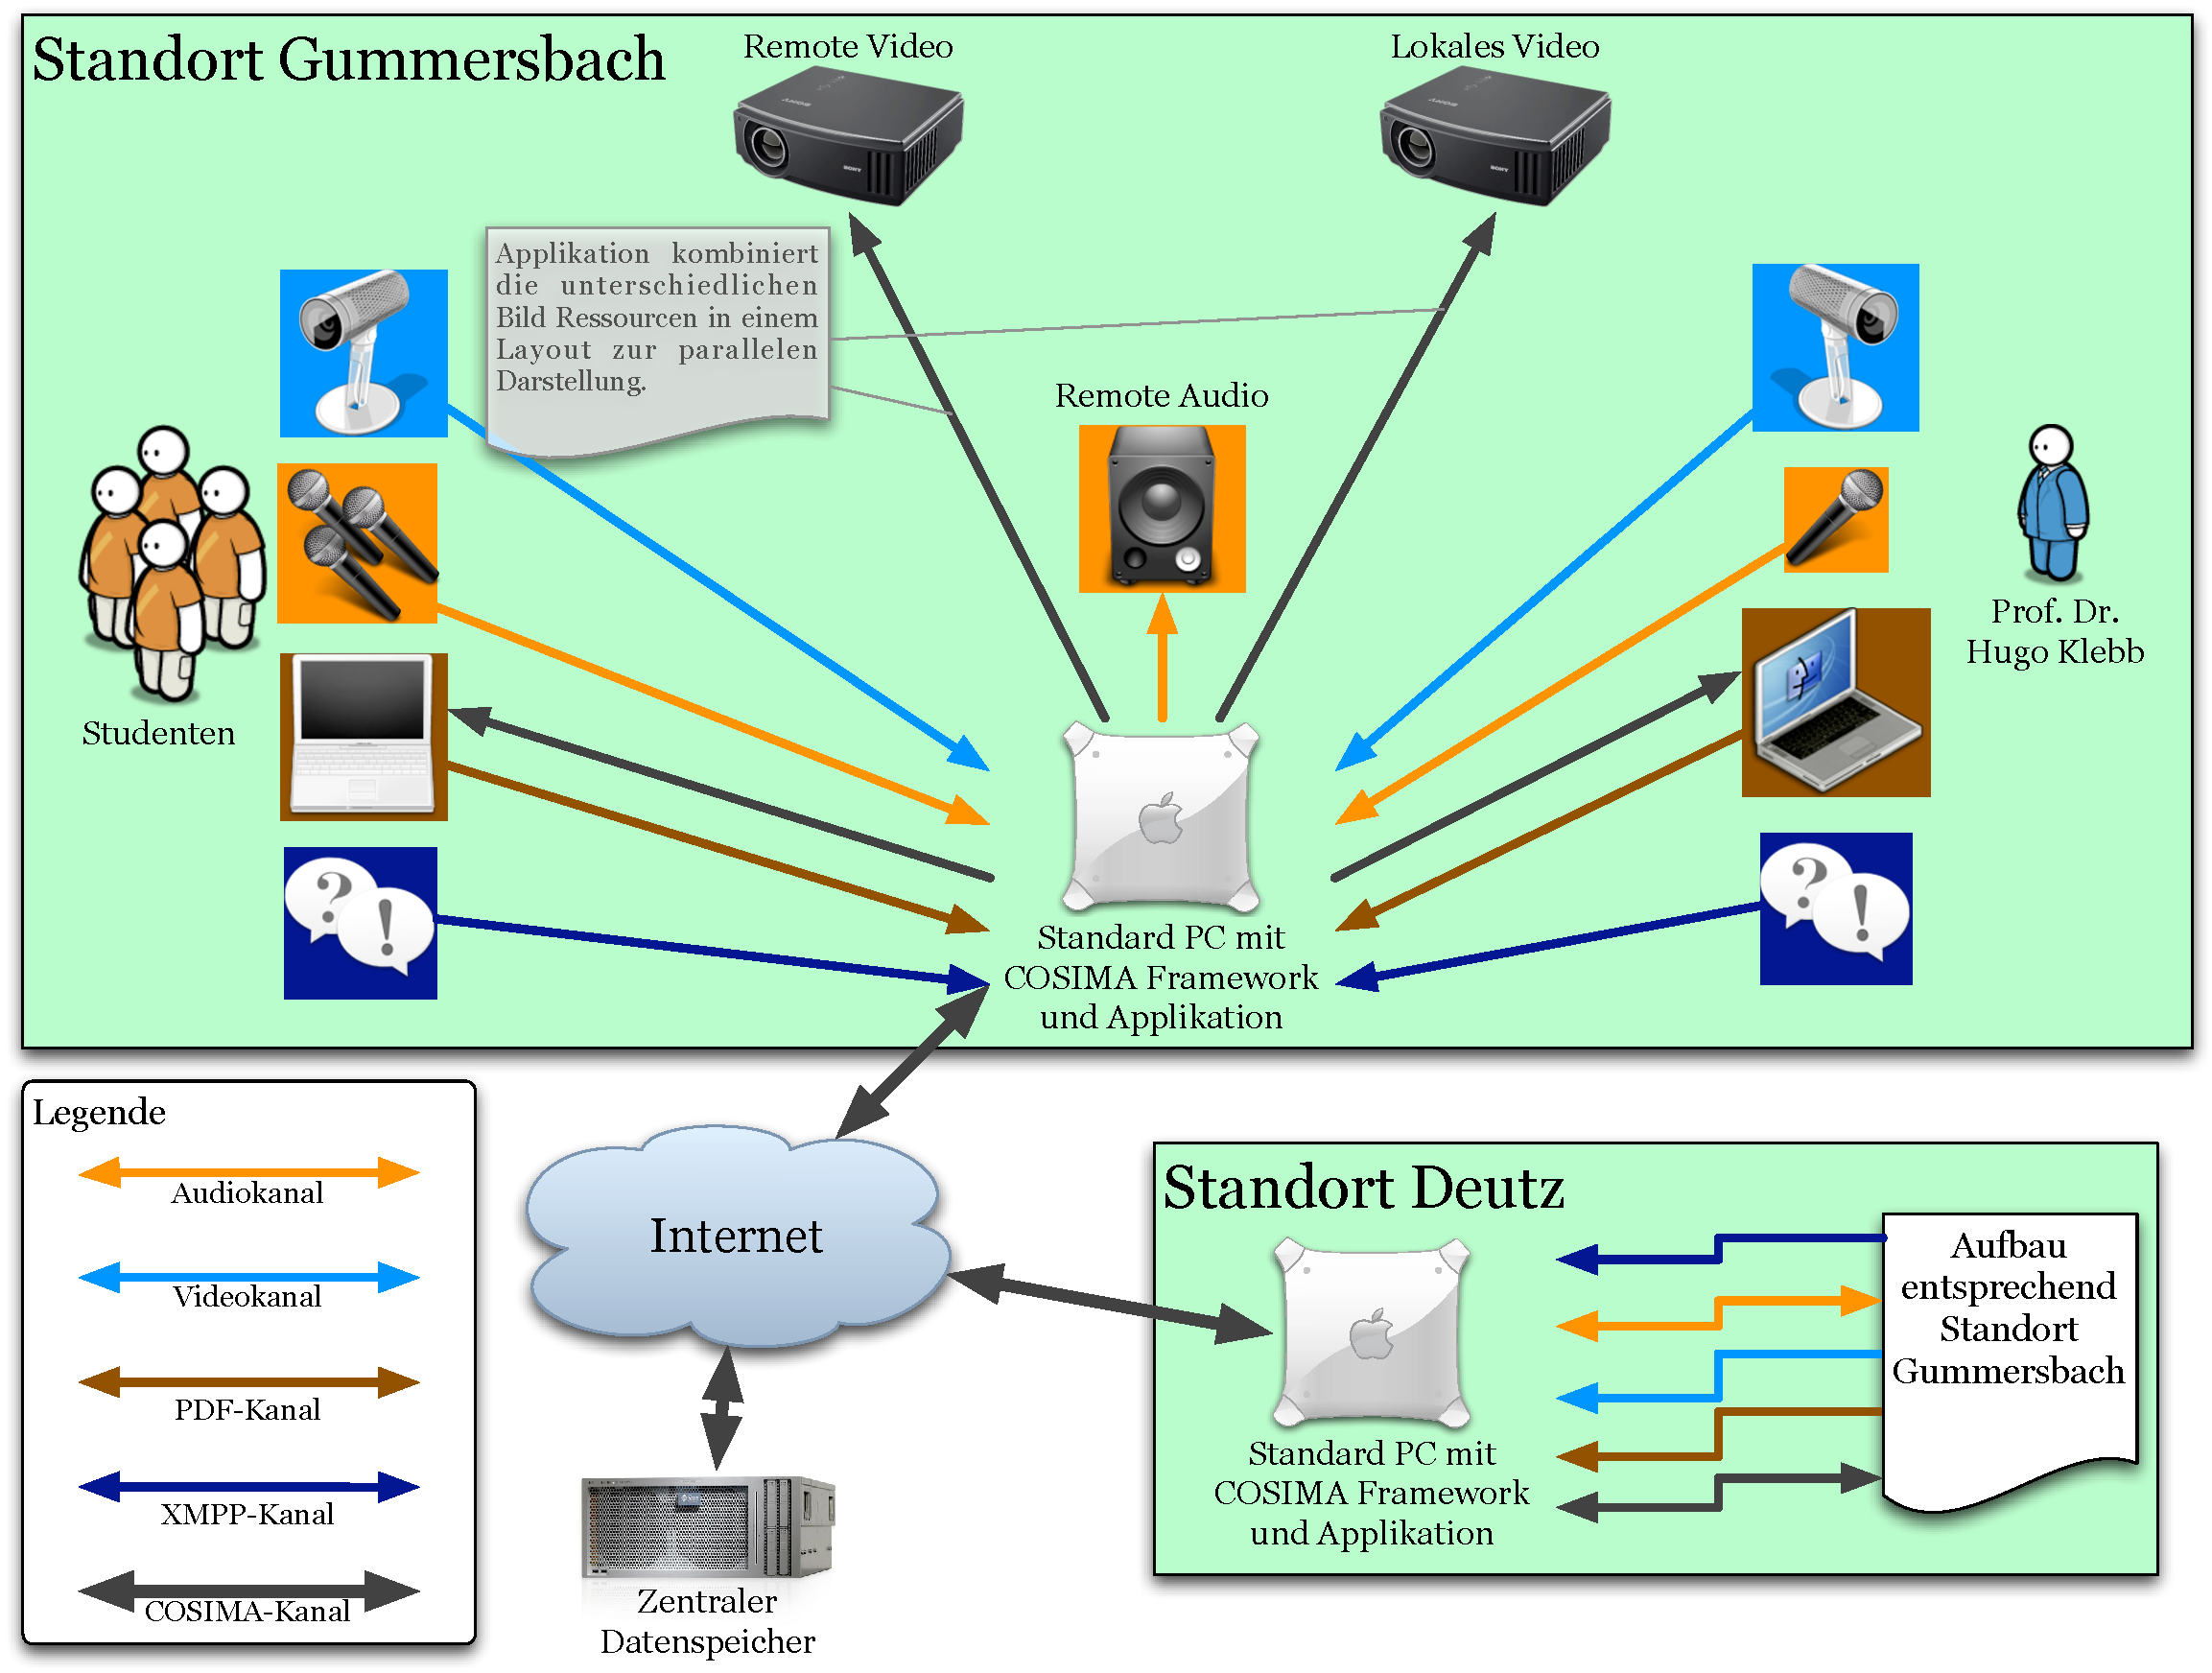
\includegraphics[width=.9\textwidth]{images/Hardware_und_Kanaele.pdf}
  \caption{Diagramm der verwendeten Hardware und Kanäle im Szenario}
  \label{fig:images_Hardware_und_Kanaele}
\end{figure}


% section beschreibung_des_szenario (end)

\section{Ablaufbeschreibung mit Personae} % (fold)
\label{sec:ablaufbeschreibung_mit_personae}

  Es ist ein sonniger Mittwoch vormittag und die Studenten des Masterstudiengangs der Medieninformatik finden sich pünktlich um 09:10 vor dem Raum 3324 an der FH Gummersbach ein. Heute steht "`Medienrezeption"' auf dem Plan. Prof. Dr. Hugo Klebb ist bereits anwesend, da er noch einige technische Vorbereitungen treffen muss. Die Veranstaltung wird zusammen mit Studenten des Studiengangs Medientechnik aus Deutz stattfinden. Das besondere dabei ist, dass die Studenten nicht körperlich anwesend sein werden, sondern durch ein neues System virtuell an der Veranstaltung teilnehmen.
  
  Kurz nachdem sich alle gesetzt haben, steht auch schon die Videoverbindung nach Deutz. Der eine Beamer zeigt ein Videobild von Prof. Dr. Julius Largo, dem Dozenten der Medientechniker und ein weiteres Videobild der Deutzer Studenten. Ebenfalls wird das Computersignal aus Deutz an die Wand geworfen. Auf einem anderen Beamer sehen die Studenten bereits die Folien von Professor Klebb.
  
  Nachdem nun alle Studenten anwesend sind und die Verbindung zwischen den Abteilungen Gummersbach und Deutz steht, beginnt die Veranstaltung. Aufgabe für heute war die Vorbereitung eines Artikels. Jeder Student sollte zu dem selben Artikel eine Textanalyse durchführen. Die Ergebnisse werden bereits im Vorfeld Online den anderen Studenten zur Verfügung gestellt, so dass jeder über das Material des anderen verfügt. Die Veranstaltung ist als seminaristischer Unterricht ausgelegt, es gibt also keinen klassischen "`Frontalunterich"'. Ziel ist es bei der Diskussion über den Artikel ein tieferes Verständnis von der Thematik zu erhalten.
  
  Die Studenten haben alle Laptops dabei und "`klinken"' sich ins FH Netz ein. Jeder kann sich in einen speziellen Chat-Raum einklinken, der nur für diese Veranstaltung gedacht ist. Sie können so parallel zu dem normalen Geschehen, weitere Punkte diskutieren oder dokumentieren. Außerdem steht ihnen auf ihrem Laptop die Möglichkeit zur Verfügung die bisherige und vergangene Veranstaltungen noch einmal anzusehen. Von dieser Möglichkeit macht denn auch direkt Vanessa gebrauch, die etwa 15 Minuten zu spät kommt. Sie stand noch im Stau auf dem Weg nach Gummersbach. Sie klingt sich in das System ein und scannt schnell über die Chat Logs, um zu sehen ob ihr etwas wichtiges entgangen ist. Zum Glück ist dem nicht so und sie kommt schnell wieder in die Veranstaltung rein.
  
  Während der Veranstaltung haben die Studenten den Text über den gesprochen wird ebenfalls auf ihren lokalen Rechnern verfügbar. Allerdings nicht einfach über das Dateisystem, sondern über die Applikation selbst. So können sie das PDF annotieren und diese Annotationen den anderen Studenten wieder zur Verfügung stellen. Auch die Textanalysen der anderen Studenten stehen ihnen über dem selben Kanal zur Verfügung.
  
  [...]
  
  Am Ende der Veranstaltung entsteht so eine Version des Textes, der von allen mit Kommentaren angereichert wurde und Querverweise zu den einzelnen Textanalysen aufweist. Zusätzlich existieren dediziert markierte Punkte im AV-Strom der Veranstaltung, die wieder auf bestimmte Textstellen linken. Angereichert mit den Chat-Logs ist so ein sehr reichhaltiges Ergebnis entstanden, auf das die Studenten und Dozenten auch später immer wieder zugreifen können.
  
\subsection{Personae} % (fold)
\label{sub:personae}

\paragraph{Dozenten} % (fold)
\label{par:dozenten}

  Die Personaebeschreibungen der Dozenten:

  \begin{itemize}

  	\item Prof. Dr. Julius Largo (Deutz)
  	\item Prof. Dr. Hugo Klebb (Gummersbach)

  \end{itemize}

% paragraph dozenten (end)

\paragraph{Studenten} % (fold)
\label{par:studenten}

  Die Personaebeschreibungen der Studenten aus Gummersbach:
  
  \begin{itemize}

  	\item   Thorsten Sommer
  	\item   Vanessa Bergmann
  	\item   Katrin Schreiber
  	\item   Uwe Gaertner
  	\item   Swen Reinhard
  	\item   Anna Müller
  	\item   Ines Gruenewald
  	\item   Nicole Eiffel
  	\item   Sara Kaiser
  	\item   Alexander Feierabend

  \end{itemize}
  
  Die Personaebeschreibungen der Studenten aus Deutz:
  
  \begin{itemize}

  	\item   Barbara Fenstermacher
  	\item   Marina Beike
  	\item   Jennifer Werner
  	\item   Christin Koehler
  	\item   Dieter Beike

  \end{itemize}
  
% paragraph studenten (end)

% subsection personae (end)

% section ablaufbeschreibung_mit_personae (end)

\section{Beschreibung der Entwicklung der benötigten Anwendung} % (fold)
\label{sec:beschreibung_der_entwicklung_der_benoetigten_anwendung}

% section beschreibung_der_entwicklung_der_benoetigten_anwendung (end)

\section{Zur Fachdomäne des Szenarios} % (fold)
\label{sec:zur_fachdomaene_des_szenarios}

- Fachdomäne KURZ skizzieren -> CSCW
- Abgrenzung des Szenarios innerhalb der Fachdomäne
- Stichworte: Virtual Classroom, Konferenzsysteme

- Begründungen warum man nichts bestehendes nimmt müssen nur skizziert werden.
  - Im Vordergrund steht die Evaluierung der Architektur
  - CampusSource stellt eine ähnliche Architektur bereit (Fokus aber nur auf Lernen) -> dort ist zumindest begründet, dass es grundsätzlich sinnvoll ist eine verteilte, dienstorientierte Architektur zu verwenden (siehe "`CampusSource Engine - Hüvelmeyer, J et al."')

% section zur_fachdomaene_des_szenarios (end)

% chapter szenario (end)
%!TEX root = /Users/dbreuer/Documents/Work/_FH/_Master/master_thesis/Main/Master Thesis.tex

\chapter{Prototypische Realisierung} % (fold)
\label{cha:prototypische_realisierung}

- Vorgehen bei der Realisierung erläutern
- Kurz (!!) auf das Santiago Projekt eingehen (da es im allerersten Schritt dazu gedient hat, eine erste funktionierende Grundlage der Architektur zu schaffen)
- Wichtige Punkte herausarbeiten
- Auf Implementierungsdetails nur an grundlegenden Stellen eingehen
- Schwierigkeiten und vor allem deren Problemlösungen darstellen
- Auswirkungen dieser Probleme/Lösungen für die Architektur
- Fokus vor allem im Text auf das Vorgehen und Wendepunkte
- Hauptteil der Quellcode
- Funktionierenden Code mit Build Tool und Dokumentation ausliefern (!!)

\section{Realisierung der Architektur} % (fold)
\label{sec:realisierung_der_architektur}

  - Santiago Projekt
  - bottom-up Ansatz
  
  
  ZUR SERVICEKOMPOSITION: Aus den in~\ref{sub:service_komposition} genannten Gründen kann auch bei der prototypische Realisierung auf die Verwendung einer existierenden Prozessbeschreibungssprache verzichtet werden.
  
\subsection{Vorgehen} % (fold)
\label{sub:vorgehen_architektur}

  - wie wurde bei der Umsetzung der Architektur vorgegangen?

% subsection vorgehen_architektur (end)
  
\subsection{Probleme und Lösungen} % (fold)
\label{sub:probleme_und_loesungen_architektur}

  - Welche Probleme sind aufgetaucht?
  - Wie wurden diese gelöst?
  - Auswirkungen auf die Architektur!
  - Workflow ohne externes Messaging System möglich!?

% subsection probleme_und_loesungen_architektur (end)

% section realisierung_der_architektur (end)

\section{Realisierung des Szenario} % (fold)
\label{sec:realisierung_des_szenario}

  - Nerstrand Projekt
  - wichtige Punkte beschreiben
  - top-down Ansatz

\subsection{Extrahierte Anforderungen} % (fold)
\label{sub:extrahierte_anforderungen}

% subsection extrahierte_anforderungen (end)

\subsection{Vorgehen} % (fold)
\label{sub:vorgehen_szenario}

  - wie wurde bei der Umsetzung des Anwendungsszenario vorgegangen?

% subsection vorgehen_szenario (end)

\subsection{Probleme und Lösungen} % (fold)
\label{sub:probleme_und_loesungen_szenario}

  - Welche Probleme sind aufgetaucht?
  - Wie wurden diese gelöst?
  - Auswirkungen auf die Architektur!

% subsection probleme_und_loesungen_szenario (end)

% section realisierung_des_szenario (end)

% chapter prototypische_realisierung (end)
\chapter{Validierung der Architektur} % (fold)
\label{cha:validierung_der_architektur}

- Vorgehen bei der Validierun darstellen
- Quellen, die dieses Vorgehen beschreiben
- Vorgehen muss noch gefunden werden (!!)
- BPEL/Orchestrierung/Choreographie mit Quellenangaben erläutern. Auswirkungen auf die ursprüngliche Konzeption der Architektur darlegen (Messaging System vs Aufruf vom Workflow System)

% chapter validierung_der_architektur (end)
\chapter{Fazit} % (fold)
\label{cha:fazit}

  In dieser Arbeit wurde die Konzeption, prototypische Implementierung sowie die Validierung einer dienstorientierten Architektur für Multimediaanwendungen behandelt. Bei der Konzeption wurde zunächst ersichtlich, dass eine dienstorientierte Architektur eine Vielzahl von unterschiedlichen Komponenten aufweist, von denen jede einzelne bereits ein gewisses Maß an Komplexität aufweist. Unter der Hinterzunahme der zusätzlichen Eigenschaften, die die Integration von Multimedia gefordert hat, entstand eine sehr komplexe Gesamtarchitektur.
  
  Durch diese hohe Komplexität war es notwendig die jeweiligen Komponenten zunächst isoliert zu betrachten und im Anschluss in den größeren Kontext einzuordnen. Durch dieses Vorgehen wurde zum einen ein sehr viel besseres Verständnis über COSIMA entwickelt, zum anderen lassen sich die Komponenten in weiteren Arbeiten einzeln leichter betrachten.
  
  In seiner Gesamtheit ist weist das COSIMA-Projekt schon ein sehr hohes Maß an Vollständigkeit auf. Die wesentlichen Aspekte sind durchweg bekannt und entsprechend diskutiert worden. Lediglich in vertikaler Richtung fehlt es Aspekten wie der Synchronisation von Medien oder der Behandlung von Metadaten noch an Tiefgang.
  
  Entsprechend der Konzeption konnte auch die Implementierung in horizontaler Ebene fast vollständig umgesetzt werden. Auch hier wurde für nachfolgende Arbeiten eine gute Grundlage geschaffen. Dies wurde vor allem auch durch das iterative Entwicklungsvorgehen und durch den Einsatz eines szenariobasierten Ansatzes begünstigt. Durch den vermehrten Einsatz von etablierten Entwurfsmustern und Entwicklungsparadigmen sowie der Verwendung der Programmiersprache Java während der Implementierung wurde auch in diesem Teil eine solide Basis für Folgeprojekte geschaffen.
  
  Es lässt sich also festhalten, dass die beiden aufgestellten Ziele im Rahmen der gestellten Aufgaben für diese Arbeit als erfüllt gelten können. Dennoch müssen einige Punkte kritisch angemerkt werden.
  
  Die Nichtverwendung einer etablierten Prozessbeschreibungssprache stellt eines der Hauptprobleme dar. Zwar erlaubt die gewählte Lösung in dieser Arbeit ein besseres Verständnis über die internen Abläufe bei der Servicekomposition für eine langfristige Weiterentwicklung sollte diese Komponente jedoch ausgetauscht werden. Stattdessen sollte die Eignung und Anpassung bestehender Lösungen weiterverfolgt werden, wie sie bereits bei \citep{samma08} begonnen wurden.
  
  Ebenfalls nur rudimentär har die Integration von Synchronisation stattgefunden. Es wurde vor allem klar, dass es sich dabei um ein sehr komplexes Themengebiet handelt. In \citep{antons09} findet aber bereits eine intensivere Auseinandersetzung mit der Einbindung von Synchronisation in das COSIMA-Projekt statt. In Zukunft sollten Arbeiten die dort gefundenen Ergebnisse mit der Implementierung aus dieser Arbeit in Einklang bringen.
  
  Der letzte Punkt der fast vollständig ignoriert wurde, ist die Betrachtung von Metadaten. Da dieser Punkt nicht zur essentiellen Funktionalität des umgesetzten Szenarios gehört, wurde bisher nur eine Schnittstelle vorgesehen. Aber in \citep{lehmann09} findet eine dedizierte Betrachtung dieser Thematik im Kontext von COSIMA statt.
  
  Zu den anderen Punkten lässt sich sagen, dass sie trotz ihres prototypischen Charakters durchaus so implementiert sind, dass sie sich auch für den Einsatz in Folgeprojekten eignen.
  
  Abschließend lässt sich festhalten, dass das gesamte COSIMA-Projekt einen innovativen und breiten Themenbereich im Rahmen der Medieninformatik bietet. Nachdem in dieser Arbeit zum ersten Mal eine funktionierende Implementierung der grundlegenden Architektur geliefert wurde, haben künftige Arbeiten in diesem Bereich eine robuste Basis zur Hand, um in den unterschiedlichen Teilbereichen des Projekts in die Tiefe zu gehen.

% chapter fazit (end)

\appendix

% \nocite{*}
\bibliography{std/bibliography}

% Einbinden des Anhangs
%!TEX root = /Users/dbreuer/Documents/Work/_FH/_Master/master_thesis/Main/Master Thesis.tex

\chapter{Weitere Listings} % (fold)
\label{cha:more_listing}

  In diesem Anhang finden sich solche Listings, die eine zu umfangreich waren, um im laufenden Text untergebracht zu werden, dennoch aber von Interesse während des Lesens der Arbeit sind und daher nicht nur auf der Begleit-CD zu finden sein sollten.

  \lstinputlisting[caption=Die \texttt{WorkflowElement}-Klasse,label=lst:workflow_element,language=Java,firstline=12]{../code/COSIMA/src/main/java/de/fhkoeln/cosima/workflow/WorkflowElement.java}

  \lstinputlisting[caption=Die \texttt{RemoteWorkflowEngine}-Klasse,label=lst:remote_workflow_engine,language=Java,firstline=12]{../code/COSIMA/src/main/java/de/fhkoeln/cosima/workflow/RemoteWorkflowEngine.java}
  
  \lstinputlisting[caption=Die vollständige \texttt{AbstractComponent}-Klasse,label=lst:abstract_component_final,language=Java,firstline=12]{../code/COSIMA/src/main/java/de/fhkoeln/cosima/components/AbstractComponent.java}
    
% chapter more_listing (end)

%!TEX root = /Users/dbreuer/Documents/Work/_FH/_Master/master_thesis/Main/Master Thesis.tex

\chapter{Architekturdarstellungen} % (fold)
\label{cha:architekturdarstellungen}

  - Auszüge aus UML-Diagrammen

% chapter architekturdarstellungen (end)

% Einbinden der Eigenständigkeitserklärung
%!TEX root = /Users/dbreuer/Documents/Work/_FH/_Master/master_thesis/Main/Master Thesis.tex

\chapter*{Erklärung}\label{chap:erklaerung}

Ich versichere, die von mir vorgelegte Arbeit selbständig verfasst zu haben.\\ \\
Alle Stellen, die wörtlich oder sinngemäß aus veröffentlichten oder nicht veröffentlichten Arbeiten anderer entnommen sind, habe ich als entnommen kenntlich gemacht. Sämtliche Quellen und Hilfsmittel, die ich für die Arbeit benutzt habe, sind angegeben.\\ \\
Die Arbeit hat mit gleichem Inhalt bzw. in wesentlichen Teilen noch keiner anderen Prüfungsgbehörde vorgelegen.

\vspace{4cm}

\begin{flushright}
  ---------------------------------------------\\
  Dirk Breuer --- Köln, den \today
\end{flushright}


% Einbindung der CC-Lizenz
%!TEX root = /Users/dbreuer/Documents/Work/_FH/_Master/master_thesis/Main/Master Thesis.tex

\newpage
\thispagestyle{empty}

% \begin{figure}[ht!]
%   \centering
%     
\includegraphics[width=.5\textwidth]{images/by-nc-nd_eu}
% \end{figure}
% 
% \vspace{1cm}
% 
%   This work is licensed under the Creative Commons Attribution-Noncommercial-No Derivative Works 3.0 Unported License. To view a copy of this license, visit \url{http://creativecommons.org/licenses/by-nc-nd/3.0/ or send a letter to} Creative Commons, 171 Second Street, Suite 300, San Francisco, California, 94105, USA.

\begin{center}
  
\includegraphics[width=.08\textwidth]{images/apple.pdf}\\
  Made on a Mac. Typesetted with \LaTeX.
\end{center}


% Unbeschriftetes Abschlussblatt
% \newpage
\thispagestyle{empty}
\mbox{}

\end{document}
